\documentclass{scrartcl}
\usepackage[utf8]{inputenc}
\usepackage{graphicx}
\usepackage{geometry}
\usepackage{titling}
\usepackage{listings}
\usepackage{amsmath}

% Configuration
\graphicspath{ {img/} }
\geometry{a4paper}
\lstset{basicstyle=\footnotesize\ttfamily,breaklines=true}
\lstset{framextopmargin=50pt}

\renewcommand\partheadstartvskip{\clearpage\null\vfil}
\renewcommand\partheadmidvskip{\par\nobreak\vskip 20pt\thispagestyle{empty}}
\renewcommand\partheadendvskip{\vfil\clearpage}
\renewcommand\raggedpart{\centering}


% Title
\title{Yet Another Stupid Compiler}
\author{
    Louis Solofrizzo\\
    \texttt{louis@ne02ptzero.me}\\
    \\
    42 Staff\\
    \texttt{staff@42.fr}
}

\pretitle{%
    \begin{center}
    \LARGE
    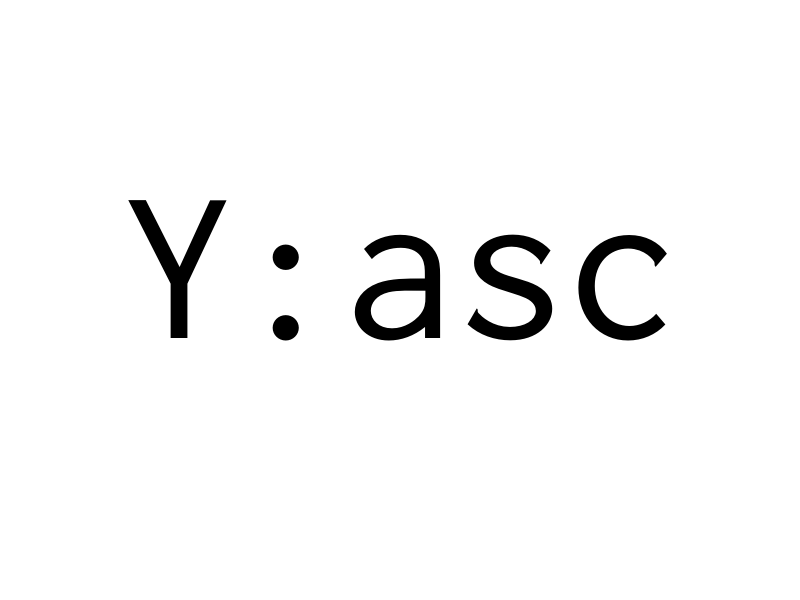
\includegraphics[scale=0.1, height=7cm]{logo}\\[\bigskipamount]
}

\posttitle{%
    \end{center}
}


% Actual document
\begin{document}

\begin{titlingpage}
    \maketitle
\end{titlingpage}


    \tableofcontents{}
    \newpage

\part{Introduction}
\part{The Y Language}
    \section{Getting Started}
    \section{Types, Operators and Expressions}
        \subsection{Variable names} \label{varnames}
            Variable names are made up of letters and digits; the first character
            must be a letter. A letter is, in this context, a character inside
            the English dictionnary, through the letters \texttt{a} to \texttt{z}.
            All other symbols from other languages / Unicode are not supported,
            and will throw an error upon reading. The underscore \texttt{\_}
            count as a letter. All variable must be in lowercase, as uppercase
            names are reserved to namespaces.
            Keywords like \texttt{if}, \texttt{else}, \texttt{struct}, etc., are
            reserved: They cannot be used as variables names.

            A variable name cannot be used twice in a scope: If such a thing
            would happen, an error will be thrown. However, different variables
            can have the same name in differents namespaces. See the \ref{namespaces}
            section for more information.
        \subsection{Namespaces} \label{namespaces}
            Namespaces are used to limit scope of functions. They must be declared
            via the keyword \texttt{def}, with brackets to delimit the scope.
            Namespaces names are made up of letters and digits; the first character
            must be a letter, in uppercase: Lowercase names are reserved to variables.

            Example of a namespace declaration:
            \begin{lstlisting}
    def Namespace_name {
        [...]
    };
            \end{lstlisting}
            Functions can be declared in a namespace:
            \begin{lstlisting}
    def Namespace_name {
        function_name(ubyte[] : str) : bool {
            [...]
            return true;
        }
    };
            \end{lstlisting}
            Any functions declared in a namespace is meant to be used with this
            namespace. In order to use a specific namespace, one must declare it:
            \begin{lstlisting}
    use Namespace_name;
            \end{lstlisting}
            The keyword \texttt{use} used with the namespace name will allow
            the call of all functions in this namespace. In order to use one
            function of this namespace, one can use an accessor on the namespace name:
            \begin{lstlisting}
    use Namespace_name.function_name;
            \end{lstlisting}
            With this declaration, any other function of this namespace used in
            code will throw an error.

            With proper usage of the keyword \texttt{use}, one can use a
            namespace's function in the following way:
            \begin{lstlisting}
    Namespace_name.function_name("Hello!");
            \end{lstlisting}

            Since namespaces are a limited scope, they can be two functions with
            the same name, in two different namespaces but they must always be used
            with a proper accessor; this way, the compiler / interpreter will
            never be confused as what function should be called.
            However, take the following example:

            \begin{lstlisting}
    def Namespace_one {
        hello(void) : void {
            print("Hello from one");
        }
    };

    def Namespace_two {
        use Namespace_one;

        hello(void) : void {
            print("Hello from two");
            hello();
        }
    };
            \end{lstlisting}
            In the \texttt{Namespace\_two} function \texttt{hello}, we call a
            function named \texttt{hello}: In this specific case, the function
            called will be the one of the current namespace, thus resulting in
            an infinite loop. If one must use a same named function in another
            namespace, a proper accessor must be used:
            \begin{lstlisting}
    def Namespace_one {
        hello(void) : void {
            print("Hello from one");
        }
    };

    def Namespace_two {
        use Namespace_one;

        hello(void) : void {
            print("Hello from two");
            Namespace_two.hello();
        }
    };

            \end{lstlisting}
            The same logic can be used for globals functions named the same as
            namespace's function:
            \begin{lstlisting}
    hello(void) : void {
        print("Hello from one");
    }

    def Namespace_two {
        hello(void) : void {
            print("Hello from two");
            hello();
        }
    };
            \end{lstlisting}
            Here, in the \texttt{Namespace\_two.hello} function, the function
            called will be itself. However, if one call the \texttt{hello} function
            from a global scope, such as \texttt{main}, the global scope will be used:
            \begin{lstlisting}
    hello(void) : void {
        print("Hello from one");
    }

    def Namespace_two {
        hello(void) : void {
            print("Hello from two");
        }
    };

    use Namespace_two;

    main(u32 : ac, ubyte[]* : av) : u32 {
        hello();
        return 0;
    }
            \end{lstlisting}
    Will return:
            \begin{lstlisting}
    > Hello from one
            \end{lstlisting}
            If one must use the \texttt{Namespace\_two} \texttt{hello} function,
            a proper accessor must be used, as shown above.


        \subsection{Data types and Sizes}
            One can use the following standard data types:

$\begin{array}{|c|c|c|}
\hline
Name & Range & Content\\
\hline
\text{ubyte} & \text{0 - 255} & \text{One byte, can be used for an ASCII-character}\\
\hline
\text{u8} & \text{0 - 255} & \text{Unsigned integer on 8 bits, same as ubyte}\\
\hline
\text{s8} & \text{-128 - 127} & \text{Signed integer on 8 bits}\\
\hline
\text{u16} & \text{0 - 65,535} & \text{Unsigned integer on 16 bits}\\
\hline
\text{s16} & \text{-32,768 - 32,767} & \text{Signed integer on 16 bits}\\
\hline
\text{u32} & \text{-2,147,483,648 - 2,147,483,647} & \text{Unsigned integer on 32 bits}\\
\hline
\text{s32} & \text{0 - 4,294,967,295} & \text{Signed integer on 32 bits}\\
\hline
\end{array}$
        \subsection{Constants} \label{const}
            One can declare a specific variable to be never changed, in any scope,
            via the keyword \texttt{\_\_const}:
            \begin{lstlisting}
    ubyte __const char = 'A';
            \end{lstlisting}
            This \texttt{char} variable can never change value; any attempt to it
            will throw an error.
            Constant variables must have a initialization value, otherwise, its
            utility is quite limited.

            The \texttt{\_\_const} keyword must always be between a variable
            type and its name.
        \subsection{Declarations}
            All variables must be declared before use, although certain
            declarations can be made implicity by content. A declaration
            specifies a type, an optionnal flag and a name.
            \begin{lstlisting}
    u32                 count, j;
    bool __const        ret = true;
            \end{lstlisting}
            Variables can be distributed among declarations in any fashion; the
            list above could well be written as
            \begin{lstlisting}
    u32         count;
    u32         j;
            \end{lstlisting}
            A variable may also be initialized in its declaration. If the name
            is followed by an equals signs and an expression, the expression
            serves as an initializer. Constant variables must be initialized,
            see the \ref{const} section for more information.

            The flag between the type and the name is implemented by the language,
            and should always be in this position.
        \subsection{Arithmetic Operators}
            The binary arithmetic operators are \texttt{+}, \texttt{-},
            \texttt{*}, \texttt{/} and the modulus operator \texttt{\%}.
            The binary operator \texttt{+} and \texttt{-} operators have the 
            same precedence, which is lower than the precedence of \texttt{*},
            \texttt{/}, and \texttt{\%}. Arithmetic operators associate left
            to right.
        \subsection{Relational and Logical Operators}
            The relational operators are

$\begin{array}{llll}
> & >= & < & <=
\end{array}$

            They all have the same precedence. Just below them in precedence are
            the equality operators:

$\begin{array}{ll}
== & !=
\end{array}$

            Relational operators have lower precedence than arithmetic operators,
            so an expression like \texttt{i < lim - 1} is taken as \texttt{i < (lim - 1)}
            , as would be expected.

            The logical operators are

$\begin{array}{ll}
\&\& & ||
\end{array}$

            Expressions connected by \texttt{\&\&} or \texttt{||} are evaluated
            left to right, and evaluation stops as soon as the truth or falsehood
            of the result is known. By definition, the numeric value of a relational
            or logical expression is 1 if the relation is true, and 0 if the relation
            is false.
        \subsection{Type Conversions}
        \subsection{Assignement Operators and Expressions}
        \subsection{Conditionnal Expressions}
        \subsection{Precedence and Order of Evaluation}
    \section{Control Flow}
        \subsection{If-Else}
        \subsection{Else-If}
        \subsection{Loops - While}
        \subsection{Loops - For}
        \subsection{Loops - Do-While}
        \subsection{Break and Continue}
    \section{Functions and Program Structure}
        \subsection{Basics}
        \subsection{External Variables}
        \subsection{Scope Rules}
        \subsection{Header Files}
        \subsection{Static Variables}
        \subsection{Recursion}
        \subsection{Preprocessor}
    \section{Pointers and Arrays}
        \subsection{Pointers and Addresses}
        \subsection{Pointers and Function Arguments}
        \subsection{Pointers and Arrays}
        \subsection{Address Arithmetic}
        \subsection{The \_\_heap argument}
        \subsection{Command-line Arguments}
    \section{Structures}
        \subsection{Basics}
        \subsection{Structures and Functions}
        \subsection{Array of Structures}
        \subsection{Pointer to Structures}
        \subsection{Packing}
    \section{Standard Library}
        \subsection{Input and Output}
        \subsection{Memory Control}
        \subsection{System Calls}
    \section{Format}
        \subsection{Comments}
        \subsection{Unicode}
        \subsection{Inline definitions}
\part{The ASC Language}
    \section{Getting Started}
    \section{Definitions}
    \section{Accessors}
        \subsection{Basics}
        \subsection{Special Accessors}
        \subsection{Constants}
    \section{Registers}
        \subsection{Infinite Registers}
        \subsection{Define a Register}
    \section{Memory}
        \subsection{Virtual Memory}
        \subsection{Paging}
        \subsection{On-Disk memory}
        \subsection{Cache}
    \section{Arithmetic}
        \subsection{Basics}
        \subsection{Comparisons}
        \subsection{Bit-Fields}
    \section{Calls}
        \subsection{Functions}
        \subsection{System Calls}
    \section{Format}
        \subsection{Comments}
        \subsection{Instructions}


\end{document}
